\part{Hiện thực hệ thống}
\label{part:ch3}
% Long code identifiers cannot be hyphenated, so this chapter allows looser inter-word spacing.
\begingroup
\sloppy

Chương này trình bày kiến trúc của hệ thống, luồng xử lý một truy vấn phân tích, sáu kịch bản truy vấn OLAP và các trang phân tích trên web. Kho dữ liệu dùng trong chương là kho đã mô tả ở Chương~\ref{part:ch2}.

\section{Kiến trúc và công nghệ}
\label{sec:architecture}
Hệ thống chia thành hai phần. Phần ngoại tuyến (\textit{offline}) dựng kho, huấn luyện mô hình và chấm điểm hàng loạt. Phần phục vụ (\textit{serving}) trả lời trang web từ kho và mô hình đã lưu. Hình~\ref{fig:system_architecture} cho thấy hai phần này và dữ liệu đi giữa chúng.

\begin{figure}[H]
	\centering
	\mermaidfile[width=0.9\linewidth, keepaspectratio]{diagrams/system_architecture.mmd}
	\caption{Kiến trúc hệ thống}
	\label{fig:system_architecture}
\end{figure}

\begin{itemize}[topsep=0pt, itemsep=1pt]
	\item \textbf{Phần ngoại tuyến:} Giao diện dòng lệnh \texttt{hcdw} có ba lệnh chính. Lệnh \texttt{hcdw etl} dựng kho từ $8$ tập tin Kaggle và nguồn ngày mô phỏng. Lệnh \texttt{hcdw train} huấn luyện mô hình, còn \texttt{hcdw score} ghi kết quả chấm điểm vào kho. Lệnh \texttt{hcdw etl -{}-score} chạy cả ba bước trong khoảng $1{,}5$ phút.
	\item \textbf{Kho dữ liệu:} Kho là một tập tin DuckDB \texttt{hc.duckdb} với ba lược đồ \texttt{staging}, \texttt{dw} và \texttt{mart}. DuckDB lưu theo cột, xử lý theo vectơ và không cần chạy máy chủ riêng. MotherDuck là bản sao trên đám mây, không bắt buộc, giúp cả nhóm truy vấn mà không phải tải dữ liệu.
	\item \textbf{Phần phục vụ:} Lệnh \texttt{hcdw serve} chạy API FastAPI tại \texttt{/api/*} và ứng dụng React một trang. API mở kho ở chế độ chỉ đọc và đọc mô hình đã lưu trong \texttt{models/}.
	\item \textbf{Mã dùng chung:} Hai phần dùng chung \texttt{src/dss/features.py}, \texttt{grading.py} và \texttt{rules.py}. Vì vậy chấm hàng loạt và chấm một hồ sơ cho cùng kết quả.
\end{itemize}

\subsection{Cơ chế vận hành}
Ba cơ chế giữ cho hệ thống ổn định và an toàn:
\begin{itemize}[topsep=0pt, itemsep=1pt]
	\item \textbf{Công bố nguyên tử:} ETL ghi vào tập tin tạm và chỉ thay kho đang dùng khi mọi kiểm tra chất lượng đều đạt (mục~\ref{sec:dq}). DuckDB chỉ cho một tiến trình ghi, nên cần tắt \texttt{hcdw serve} trước khi chạy \texttt{hcdw etl} hoặc \texttt{hcdw score}.
	\item \textbf{An toàn truy vấn:} Trình duyệt không bao giờ gửi câu SQL. API kiểm tra tên chiều và tên thước đo theo danh sách cho phép \texttt{DIMENSIONS} và \texttt{MEASURES}, còn giá trị lọc đi qua tham số gán.
	\item \textbf{Bộ nhớ đệm:} Kho là ảnh chụp tĩnh cho tới lần ETL sau, nên các truy vấn của \textbf{Overview}, \textbf{Grades \& model}, \textbf{Rules}, \textbf{SQL queries} và phần số liệu tổng thể của \textbf{Explorer} được nhớ bằng \texttt{lru\_cache}. Truy vấn khối dữ liệu của \textbf{Analytics} không dùng bộ nhớ đệm.
\end{itemize}

\begin{table}[H]
	\centering
	\caption{Công nghệ sử dụng trong hệ thống}
	\label{tab:tech-stack}
	\footnotesize
	\begin{tabular}{p{3.4cm} p{5.4cm} p{6.6cm}}
		\toprule
		\textbf{Tầng}     & \textbf{Công nghệ}                             & \textbf{Vai trò}                                                                                                 \\
		\midrule
		Lưu trữ và OLAP   & DuckDB (tập tin cục bộ), MotherDuck (tùy chọn) & Lưu bảng chiều, bảng sự kiện và khung nhìn; thực thi truy vấn tổng hợp.                                          \\
		ETL               & Python 3.11+, pandas, DuckDB SQL, Typer        & Đọc CSV, làm sạch, gộp, nạp kho và cung cấp giao diện dòng lệnh \texttt{hcdw}.                                   \\
		Dịch vụ           & FastAPI, Uvicorn, pydantic                     & Cung cấp API JSON, kiểm tra yêu cầu và tham số hóa truy vấn.                                                     \\
		Giao diện         & React 18, TypeScript, Tailwind CSS, Recharts   & Vẽ biểu đồ, bảng và các sơ đồ thiết kế.                                                                          \\
		Hỗ trợ quyết định & LightGBM, scikit-learn, SHAP                   & Ước lượng xác suất vỡ nợ, hiệu chỉnh bằng hồi quy đơn điệu (\textit{isotonic regression}) và giải thích kết quả. \\
		Kiểm thử          & pytest                                         & Kiểm thử ETL, API và DSS; báo cáo chất lượng sau mỗi lần chạy.                                                   \\
		\bottomrule
	\end{tabular}
\end{table}

\section{Luồng xử lý một truy vấn OLAP}
\label{sec:request-flow}
Hình~\ref{fig:flow_request} mô tả điều xảy ra khi người dùng đổi khối dữ liệu trên trang \textbf{Analytics}.

\begin{figure}[H]
	\centering
	\mermaidfile[width=0.92\linewidth, keepaspectratio]{diagrams/flow_request.mmd}
	\caption{Luồng xử lý một truy vấn OLAP}
	\label{fig:flow_request}
\end{figure}

\begin{enumerate}[topsep=0pt, itemsep=1pt]
	\item Người dùng thêm một điều kiện lọc, hoặc bấm \textbf{Interval}, $\blacktriangle$/$\blacktriangledown$, $\times$, $+$ hay $\rightleftarrows$. Trạng thái của trang được ghi vào tham số \texttt{?state=} trên URL, nên có thể chia sẻ bằng đường dẫn.
	\item Tùy phần bị ảnh hưởng, trang gửi $5$ yêu cầu \texttt{POST /api/analytics/cube} (khi đổi bộ lọc \textbf{Cohort}), $3$ yêu cầu (khi đổi \textbf{Interval} cho ba biểu đồ thời gian) hoặc $1$ yêu cầu (khi đổi \textbf{Split by} hay cấu hình bảng \textbf{Cube}); các kết quả đã có trong bộ nhớ đệm phía trình duyệt không phải gửi lại.
	\item API kiểm tra thân yêu cầu bằng pydantic; sai kiểu dữ liệu thì trả mã $422$.
	\item Mã \texttt{cube.py} kiểm tra tên chiều và thước đo theo danh sách cho phép, tối đa $2$ chiều hàng và $1$ chiều cột, không lặp chiều; sai thì trả mã $400$.
	\item API chạy một câu \mintinline[fontsize=\small]{sql}|GROUP BY GROUPING SETS (...)| trên \texttt{mart.v\_application\_wide}. Kết quả gồm các ô, tổng phụ và tổng chung.
	\item Trình duyệt vẽ lại biểu đồ và bảng. Bấm vào một ô mở trang \textbf{Explorer} với nhóm hồ sơ tương ứng (\textit{drill-through}).
\end{enumerate}

\section{Truy vấn phân tích trực tuyến (OLAP)}
\label{sec:olap}

\subsection{Khối dữ liệu và các phép OLAP trên trang Analytics}
Khối dữ liệu của trang \textbf{Analytics} dựa trên khung nhìn \texttt{mart.v\_application\_wide}. Khung nhìn này nối \texttt{fact\_loan\_application} với các bảng chiều và kết quả chấm điểm. Các chiều gồm thuộc tính khách hàng, lịch sử tín dụng, hợp đồng, vùng, hạng, quyết định và phân cấp thời gian năm $\rightarrow$ quý $\rightarrow$ tháng theo ngày nộp hồ sơ. Ngày nộp hồ sơ là dữ liệu mô phỏng (mục~\ref{sec:time}), nên trục thời gian chỉ minh họa phép OLAP, không mang ý nghĩa nghiệp vụ. Hình~\ref{fig:olap_operations} và Bảng~\ref{tab:olap-ui} cho thấy mỗi phép OLAP ứng với điều khiển nào trên giao diện và phần nào của câu SQL.

\begin{figure}[H]
	\centering
	\mermaidfile[width=\linewidth, keepaspectratio]{diagrams/olap_operations.mmd}
	\caption{Các phép OLAP trên trang \textbf{Analytics}}
	\label{fig:olap_operations}
\end{figure}

\begin{table}[H]
	\centering
	\caption{Ánh xạ phép OLAP sang giao diện, yêu cầu và SQL}
	\label{tab:olap-ui}
	\footnotesize
	\begin{tabular}{p{2.6cm} p{4.8cm} p{3cm} p{4.6cm}}
		\toprule
		\textbf{Phép OLAP}                                            & \textbf{Trên giao diện}                                                                                                                 & \textbf{Trường trong yêu cầu}      & \textbf{SQL}                                                                      \\
		\midrule
		Cắt lát và cắt khối (\textit{slice}, \textit{dice})           & Điều kiện lọc trên thanh \textbf{Cohort}                                                                                                & \texttt{conditions[]}              & \mintinline[fontsize=\footnotesize]{sql}|WHERE ... IN (...)|, giá trị qua tham số \\
		Cuộn lên, khoan xuống (\textit{roll-up}, \textit{drill-down}) & \textbf{Interval} Year / Quarter / Month; $\blacktriangle$/$\blacktriangledown$ trên chiều thời gian; $\times$ bỏ chiều; $+$ thêm chiều & các mức trong \texttt{rows[]}      & Tiền tố của \mintinline[fontsize=\footnotesize]{sql}|GROUPING SETS| tạo tổng phụ  \\
		Xoay (\textit{pivot})                                         & Nút $\rightleftarrows$                                                                                                                  & đổi \texttt{rows} và \texttt{cols} & --                                                                                \\
		Chọn thước đo                                                 & Ô chọn \textbf{Measure}                                                                                                                 & \texttt{measure}                   & Biểu thức trong \texttt{MEASURES}                                                 \\
		Khoan xuyên (\textit{drill-through})                          & Bấm một ô hoặc một cột                                                                                                                  & --                                 & Mở \textbf{Explorer} với các điều kiện tương ứng                                  \\
		\bottomrule
	\end{tabular}
\end{table}

\subsection{Kịch bản truy vấn OLAP}
\label{sec:olap-scenarios}
Hệ thống lưu sáu truy vấn mẫu trong thư mục \texttt{src/sql/olap/}, mỗi truy vấn minh họa một kỹ thuật OLAP. Thẻ \textbf{SQL queries} của trang \textbf{Analytics} chạy các truy vấn này qua \texttt{GET /api/olap/\{name\}}. Kịch bản $1$--$4$ và $6$ tính trên khoản vay lịch sử ($307.511$ hồ sơ, điều kiện \mintinline[fontsize=\small]{sql}|WHERE is_train|). Kịch bản $5$ tính trên \texttt{fact\_bureau\_credit}. Mọi kết quả dưới đây tính trên kho dữ liệu thật.

\subsubsection*{Kịch bản 1: Cuộn lên theo nhóm tuổi và khung thu nhập}
\paragraph{Mục đích:} Trưởng phòng rủi ro xem tỷ lệ vỡ nợ và khoản vay bình quân ở ba mức: từng tổ hợp nhóm tuổi $\times$ khung thu nhập, tổng phụ của mỗi nhóm tuổi và tổng chung.
\paragraph{Hiện thực:} Mã nguồn~\ref{sql:olap_rollup} là tập tin \texttt{src/sql/olap/}\allowbreak\texttt{01\_rollup\_age\_income.sql}. Truy vấn dùng \mintinline[fontsize=\small]{sql}|GROUP BY ROLLUP (age_bucket, income_bracket)| và hàm \mintinline[fontsize=\small]{sql}|GROUPING()| để gắn nhãn \mintinline[fontsize=\small]{sql}|'ALL'| cho dòng tổng.

\begin{listing}[H]
	\footnotesize
	\begin{minted}[linenos, breaklines]{sql}
-- OLAP: ROLL-UP along the customer hierarchy (age bucket -> income bracket -> all).
-- Subtotal rows have NULL in the rolled-up column; GROUPING() tells you which level a row is.
SELECT
    CASE WHEN GROUPING(age_bucket) = 1 THEN 'ALL' ELSE age_bucket END         AS age_bucket,
    CASE WHEN GROUPING(income_bracket) = 1 THEN 'ALL' ELSE income_bracket END AS income_bracket,
    COUNT(*)                         AS n_applications,
    ROUND(AVG(target) * 100, 2)      AS default_rate_pct,
    ROUND(AVG(amt_credit), 0)        AS avg_credit
FROM mart.v_application_wide
WHERE is_train
GROUP BY ROLLUP (age_bucket, income_bracket)
ORDER BY GROUPING(age_bucket), age_bucket, GROUPING(income_bracket), income_bracket;
\end{minted}
	\caption{Truy vấn cuộn lên theo nhóm tuổi và khung thu nhập}
	\label{sql:olap_rollup}
\end{listing}

\paragraph{Kết quả:} Tỷ lệ vỡ nợ giảm dần theo tuổi: $12{,}29\%$ ở nhóm $18$--$24$, $10{,}66\%$ ở nhóm $25$--$34$, $5{,}42\%$ ở nhóm $55$--$64$ và $3{,}66\%$ ở nhóm $65+$. Tỷ lệ chung là $8{,}07\%$. Trong mọi nhóm tuổi, khung thu nhập trên $300$ nghìn có tỷ lệ vỡ nợ thấp hơn khung dưới $100$ nghìn, ví dụ $9{,}32\%$ so với $13{,}13\%$ ở nhóm $18$--$24$. Khoản vay bình quân tăng theo thu nhập, ví dụ từ $410.681$ lên $964.268$ (đơn vị tiền gốc) ở nhóm $35$--$44$.

\subsubsection*{Kịch bản 2: Khối đầy đủ theo loại hợp đồng và giới tính}
\paragraph{Mục đích:} Người dùng xem mọi tổ hợp tổng phụ giữa loại hợp đồng (vay tiền mặt \mintinline[fontsize=\small]{sql}|'Cash loans'| và tín dụng quay vòng \mintinline[fontsize=\small]{sql}|'Revolving loans'|) và giới tính, kèm trung vị tỷ lệ trả góp trên thu nhập.
\paragraph{Hiện thực:} Mã nguồn~\ref{sql:olap_cube} là tập tin \texttt{src/sql/olap/}\allowbreak\texttt{02\_cube\_contract\_gender.sql}. Toán tử \mintinline[fontsize=\small]{sql}|CUBE (contract_type, gender)| tính cả $2^2 = 4$ mức gộp trong một câu lệnh.

\begin{listing}[H]
	\footnotesize
	\begin{minted}[linenos, breaklines]{sql}
-- OLAP: CUBE over contract type x gender (every combination of subtotals).
-- GROUPING() = 1 marks a subtotal level; it also sorts the subtotal rows after their members.
SELECT
    CASE WHEN GROUPING(contract_type) = 1 THEN 'ALL' ELSE contract_type END AS contract_type,
    CASE WHEN GROUPING(gender) = 1 THEN 'ALL' ELSE gender END               AS gender,
    COUNT(*)                         AS n_applications,
    ROUND(AVG(target) * 100, 2)      AS default_rate_pct,
    ROUND(MEDIAN(debt_to_income), 3) AS median_dti
FROM mart.v_application_wide
WHERE is_train
GROUP BY CUBE (contract_type, gender)
ORDER BY GROUPING(contract_type), contract_type, GROUPING(gender), gender;
\end{minted}
	\caption{Truy vấn khối đầy đủ theo loại hợp đồng và giới tính}
	\label{sql:olap_cube}
\end{listing}

\paragraph{Kết quả:} Khách hàng nam có tỷ lệ vỡ nợ $10{,}14\%$, cao hơn $7{,}00\%$ của khách hàng nữ. Vay tiền mặt chiếm $278.232$ trên $307.511$ hồ sơ và có tỷ lệ vỡ nợ $8{,}35\%$, cao hơn $5{,}48\%$ của tín dụng quay vòng. Trung vị tỷ lệ trả góp trên thu nhập là $0{,}172$ với vay tiền mặt và $0{,}100$ với tín dụng quay vòng. Nhóm giới tính \mintinline[fontsize=\small]{sql}|'Unknown'| chỉ có $4$ hồ sơ nên không đủ để kết luận.

\subsubsection*{Kịch bản 3: Khoan xuống từ nhóm tuổi tới nghề nghiệp}
\paragraph{Mục đích:} Nhóm tuổi $25$--$34$ có tỷ lệ vỡ nợ $10{,}66\%$, cao hơn mức chung. Chuyên viên khoan xuống từ nhóm tuổi này tới loại thu nhập và nghề nghiệp để tìm cụm rủi ro cụ thể.
\paragraph{Hiện thực:} Mã nguồn~\ref{sql:olap_drilldown} là tập tin \texttt{src/sql/olap/}\allowbreak\texttt{03\_drilldown\_age\_occupation.sql}. Truy vấn cố định \mintinline[fontsize=\small]{sql}|age_bucket = '25-34'| và bỏ các nhóm quá nhỏ bằng \mintinline[fontsize=\small]{sql}|HAVING COUNT(*) >= 30|.

\begin{listing}[H]
	\footnotesize
	\begin{minted}[linenos, breaklines]{sql}
-- OLAP: DRILL-DOWN from one age bucket into employment type, then occupation.
-- Change the slice value to drill into another member.
SELECT
    income_type,
    occupation_type,
    COUNT(*)                    AS n_applications,
    ROUND(AVG(target) * 100, 2) AS default_rate_pct
FROM mart.v_application_wide
WHERE is_train
  AND age_bucket = '25-34'
GROUP BY income_type, occupation_type
HAVING COUNT(*) >= 30
ORDER BY default_rate_pct DESC;
\end{minted}
	\caption{Truy vấn khoan xuống từ nhóm tuổi tới nghề nghiệp}
	\label{sql:olap_drilldown}
\end{listing}

\paragraph{Kết quả:} Truy vấn trả về $52$ tổ hợp loại thu nhập $\times$ nghề nghiệp. Tổ hợp rủi ro nhất là \mintinline[fontsize=\small]{sql}|'Commercial associate'| -- \mintinline[fontsize=\small]{sql}|'Cleaning staff'| với $23{,}38\%$, nhưng chỉ có $77$ hồ sơ. Tiếp theo là \mintinline[fontsize=\small]{sql}|'Working'| -- \mintinline[fontsize=\small]{sql}|'Low-skill Laborers'| ($21{,}17\%$, $548$ hồ sơ) và \mintinline[fontsize=\small]{sql}|'Working'| -- \mintinline[fontsize=\small]{sql}|'Security staff'| ($17{,}17\%$, $833$ hồ sơ). Nhóm lớn nhất là \mintinline[fontsize=\small]{sql}|'Working'| -- \mintinline[fontsize=\small]{sql}|'Laborers'| với $11.823$ hồ sơ và tỷ lệ $13{,}86\%$. Tổ hợp an toàn nhất là \mintinline[fontsize=\small]{sql}|'State servant'| -- \mintinline[fontsize=\small]{sql}|'Secretaries'| với $3{,}26\%$.

\subsubsection*{Kịch bản 4: Cắt lát, cắt khối và xoay ma trận lịch sử tín dụng}
\paragraph{Mục đích:} Người dùng cắt lát theo vay tiền mặt, cắt khối lấy các khách có lịch sử tín dụng ngoài, rồi xoay kết quả. Ma trận có hàng là số khoản tín dụng ngoài đang hoạt động và cột là nhóm số ngày quá hạn tối đa.
\paragraph{Hiện thực:} Mã nguồn~\ref{sql:olap_pivot} là tập tin \texttt{src/sql/olap/}\allowbreak\texttt{04\_slice\_dice\_credit\_history.sql}, dùng cú pháp \mintinline[fontsize=\small]{sql}|PIVOT| của DuckDB.

\begin{listing}[H]
	\footnotesize
	\begin{minted}[linenos, breaklines]{sql}
-- OLAP: SLICE (cash loans only) + DICE (customers with bureau history, two DPD buckets)
-- then PIVOT the result: credit-history bucket rows x DPD bucket columns.
PIVOT (
    SELECT bureau_active_bucket, max_dpd_bucket, target
    FROM mart.v_application_wide
    WHERE is_train
      AND contract_type = 'Cash loans'
      AND bureau_active_bucket <> 'No bureau record'
)
ON max_dpd_bucket IN ('No DPD', '1-30', '31-60', '61-90', '90+')   -- fixed column order
USING ROUND(AVG(target) * 100, 2)
GROUP BY bureau_active_bucket
ORDER BY bureau_active_bucket;
\end{minted}
	\caption{Truy vấn cắt lát, cắt khối và xoay ma trận lịch sử tín dụng}
	\label{sql:olap_pivot}
\end{listing}

\paragraph{Kết quả:} Nhìn chung, rủi ro tăng theo cả hai chiều. Ở mọi nhóm quá hạn, khách có từ $6$ khoản đang hoạt động trở lên rủi ro nhất, với tỷ lệ $11{,}12\%$--$16{,}77\%$. Khách không còn khoản nào đang hoạt động có tỷ lệ $4{,}40\%$--$11{,}31\%$. Khách chưa từng quá hạn có tỷ lệ thấp nhất ($4{,}40\%$--$11{,}12\%$), còn nhóm quá hạn $61$--$90$ ngày cao nhất ($11{,}31\%$--$16{,}77\%$). Nhóm quá hạn trên $90$ ngày ($8{,}16\%$--$13{,}89\%$) lại thấp hơn nhóm $61$--$90$ ngày. Vì vậy số ngày quá hạn trong quá khứ không làm tăng rủi ro theo đường thẳng và cần dùng cùng các chỉ số khác.

\subsubsection*{Kịch bản 5: Cuộn lên theo thời gian trên khoản tín dụng ngoài}
\paragraph{Mục đích:} Ban điều hành xem số khoản tín dụng ngoài được mở và tỷ lệ còn hoạt động theo quý, theo năm và tổng chung.
\paragraph{Hiện thực:} Mã nguồn~\ref{sql:olap_trend} là tập tin \texttt{src/sql/olap/}\allowbreak\texttt{05\_bureau\_trend\_by\_quarter.sql}. Truy vấn nối \texttt{fact\_bureau\_credit} với \texttt{dim\_time} theo vai trò ngày mở (\texttt{open\_date\_key}) và với chiều gom \texttt{dim\_bureau\_category}.

\begin{listing}[H]
	\footnotesize
	\begin{minted}[linenos, breaklines]{sql}
-- OLAP: time roll-up on fact_bureau_credit (quarter -> year -> all) using dim_time,
-- with the credit status taken from the dim_bureau_category junk dimension.
SELECT
    CASE WHEN GROUPING(t.year) = 1 THEN 'ALL' ELSE CAST(t.year AS VARCHAR) END       AS year,
    CASE WHEN GROUPING(t.quarter) = 1 THEN 'ALL' ELSE 'Q' || t.quarter END           AS quarter,
    COUNT(*)                                                   AS credits_opened,
    COUNT(*) FILTER (WHERE g.credit_active = 'Active')         AS still_active,
    ROUND(SUM(b.amt_credit_sum) / 1e6, 2)                      AS credit_sum_millions
FROM dw.fact_bureau_credit b
JOIN dw.dim_time t            ON t.date_key = b.open_date_key
JOIN dw.dim_bureau_category g USING (bureau_category_key)
GROUP BY ROLLUP (t.year, t.quarter)
ORDER BY GROUPING(t.year), t.year, GROUPING(t.quarter), t.quarter;
\end{minted}
	\caption{Truy vấn cuộn lên theo năm và quý trên khoản tín dụng ngoài}
	\label{sql:olap_trend}
\end{listing}

\paragraph{Kết quả:} Các khoản tín dụng ngoài trải từ quý 2/2007 đến quý 2/2018. Số khoản mở mỗi năm tăng từ $253.565$ năm 2013 lên $303.198$ năm 2014 và đạt đỉnh $304.696$ năm 2015. Sau đó số khoản giảm còn $174.307$ năm 2016, $43.187$ năm 2017 và $2.056$ năm 2018. Tỷ lệ còn hoạt động tăng ở các năm gần ngày mốc: $9{,}9\%$ năm 2010, $60{,}1\%$ năm 2015 và $75{,}1\%$ năm 2017. Ngày mở bằng ngày nộp hồ sơ cộng \texttt{DAYS\_CREDIT}, mà \textbf{ngày nộp hồ sơ là dữ liệu mô phỏng}. Vì vậy hình dạng xu hướng theo năm phụ thuộc cách sinh ngày và không có ý nghĩa nghiệp vụ. Quan hệ đáng tin hơn dựa trên độ lệch ngày thật của Kaggle: $78{,}0\%$ khoản mở trong vòng một năm trước ngày nộp còn hoạt động. Với khoản mở từ năm năm trước trở lên, tỷ lệ này chỉ khoảng $10\%$.

\subsubsection*{Kịch bản 6: Xếp hạng nghề nghiệp rủi ro bằng hàm cửa sổ}
\paragraph{Mục đích:} Hệ thống lấy ra ba nghề nghiệp có tỷ lệ vỡ nợ cao nhất trong mỗi nhóm tuổi. Danh sách này giúp trưởng phòng rủi ro xem xét các điều kiện thẩm định chặt hơn cho những nhóm đó.
\paragraph{Hiện thực:} Mã nguồn~\ref{sql:olap_ranking} là tập tin \texttt{src/sql/olap/}\allowbreak\texttt{06\_rank\_riskiest\_occupations.sql}. Truy vấn dùng hàm cửa sổ \mintinline[fontsize=\small]{sql}|RANK()|, phân hoạch theo \texttt{age\_bucket} và sắp theo \mintinline[fontsize=\small]{sql}|AVG(target) DESC|, rồi chỉ giữ nhóm có ít nhất $30$ hồ sơ.

\begin{listing}[H]
	\footnotesize
	\begin{minted}[linenos, breaklines]{sql}
-- OLAP: RANKING with a window function - the 3 riskiest occupations inside each age bucket.
-- Small groups are skipped (n >= 30 labelled applications) so the rate is not just noise.
SELECT
    age_bucket,
    occupation_type,
    n_labelled,
    default_rate_pct,
    rank_in_bucket
FROM (
    SELECT
        age_bucket,
        occupation_type,
        COUNT(*)                                                    AS n_labelled,
        ROUND(AVG(target) * 100, 2)                                 AS default_rate_pct,
        RANK() OVER (PARTITION BY age_bucket ORDER BY AVG(target) DESC) AS rank_in_bucket
    FROM mart.v_application_wide
    WHERE is_train
    GROUP BY age_bucket, occupation_type
    HAVING COUNT(*) >= 30
)
WHERE rank_in_bucket <= 3
ORDER BY age_bucket, rank_in_bucket;
\end{minted}
	\caption{Truy vấn xếp hạng ba nghề nghiệp rủi ro nhất mỗi nhóm tuổi}
	\label{sql:olap_ranking}
\end{listing}

\paragraph{Kết quả:} \mintinline[fontsize=\small]{sql}|'Low-skill Laborers'| đứng đầu ở $5$ trên $6$ nhóm tuổi, với tỷ lệ từ $13{,}67\%$ đến $20{,}16\%$. Các vị trí tiếp theo chủ yếu là \mintinline[fontsize=\small]{sql}|'Drivers'|, \mintinline[fontsize=\small]{sql}|'Security staff'| và \mintinline[fontsize=\small]{sql}|'Cleaning staff'|. Hai kết quả cần đọc thận trọng vì cỡ mẫu nhỏ. \mintinline[fontsize=\small]{sql}|'IT staff'| đứng thứ hai ở nhóm $45$--$54$ với $56$ hồ sơ. \mintinline[fontsize=\small]{sql}|'Medicine staff'| đứng đầu nhóm $65+$ với $72$ hồ sơ và tỷ lệ $6{,}94\%$, vẫn thấp hơn mức chung $8{,}07\%$. Hai trường hợp này cho thấy vì sao truy vấn cần ngưỡng cỡ mẫu tối thiểu.

\subsection{Hiệu năng truy vấn}
Mỗi truy vấn khối dữ liệu của trang \textbf{Analytics} mất khoảng $15$--$60$ ms trên $356.255$ hồ sơ và không dùng bộ nhớ đệm. Các truy vấn đọc khác của API được nhớ bằng \texttt{lru\_cache}, nên lần gọi lặp lại không phải chạy lại SQL. DuckDB đủ nhanh cho quy mô dữ liệu của bài toán mà không cần máy chủ cơ sở dữ liệu riêng.

\section{Giao diện trực quan hóa (dashboard)}
\label{sec:dashboard}
Ứng dụng web có năm trang ở menu chính: \textbf{Overview}, \textbf{Analytics}, \textbf{Explorer}, \textbf{Application details} và \textbf{Playground}. Hai trang tham khảo \textbf{Grades \& model} và \textbf{Architecture} nằm ở chân thanh bên. Mọi số tổng hợp trên web tính trên mọi hồ sơ (đã chấm), tức $356.255$ hồ sơ. Riêng các chỉ số cần kết quả trả nợ, như tỷ lệ vỡ nợ, chỉ tính trên $307.511$ khoản vay lịch sử. Mục này trình bày ba trang phân tích; các trang \textbf{Application details}, \textbf{Playground} và \textbf{Grades \& model} được trình bày ở Chương~\ref{part:ch4}.

\subsection{Trang Overview}
Trang \textbf{Overview} là điểm vào đầu tiên, cho cái nhìn tổng thể về danh mục. Hình~\ref{fig:page_overview} là ảnh chụp trang với cấu hình mặc định gồm ba phần:

\begin{itemize}[topsep=0pt, itemsep=1pt]
	\item \textbf{Biểu đồ ô vuông (\textit{waffle}):} Khung \textbf{Out of every 100 applications} chia $100$ ô theo quyết định và kết quả trên khoản vay lịch sử. Nhóm Duyệt (\textbf{Approve}) chiếm $52\%$ và có $3{,}4\%$ vỡ nợ. Nhóm Thẩm định thêm (\textbf{Manual review}) chiếm $39\%$ và có $9{,}9\%$ vỡ nợ. Nhóm Từ chối (\textbf{Reject}) chiếm $9\%$ và có $28{,}0\%$ vỡ nợ. Bấm một ô mở \textbf{Explorer} với nhóm đó.
	\item \textbf{Năm ô KPI:} Dải \textbf{All applications} tính trên mọi hồ sơ và không theo bộ lọc nào. \textbf{Default rate} là $8{,}07\%$ (chỉ trên khoản vay lịch sử), \textbf{Total credit} là $209{,}4$ tỷ (đơn vị tiền gốc) và \textbf{Credit at risk} là $15{,}76$ tỷ. \textbf{Approval rate} là $51{,}86\%$ và \textbf{Manual review rate} là $39{,}54\%$.
	\item \textbf{Phân tích theo phân khúc:} Ô chọn \textbf{Group by} có $13$ thuộc tính, mặc định là \texttt{credit\_history\_status}, và được lưu trong tham số \texttt{?dim=}. Ô này điều khiển biểu đồ \textbf{Default rate by segment} và bảng \textbf{Segment size}. Bấm một cột mở \textbf{Explorer} với nhóm đó làm điều kiện lọc.
\end{itemize}

Tỷ lệ duyệt trên biểu đồ ô vuông ($52{,}07\%$) khác ô KPI ($51{,}86\%$) vì biểu đồ ô vuông tính trên khoản vay lịch sử, còn ô KPI tính trên mọi hồ sơ (đã chấm). Với cấu hình mặc định, biểu đồ phân khúc cho thấy khách đang quá hạn ở tổ chức khác có tỷ lệ vỡ nợ $16{,}11\%$. Khách không có lịch sử tín dụng ngoài có tỷ lệ $10{,}12\%$, còn khách có lịch sử sạch có tỷ lệ $7{,}62\%$.

\begin{figure}[H]
	\centering
	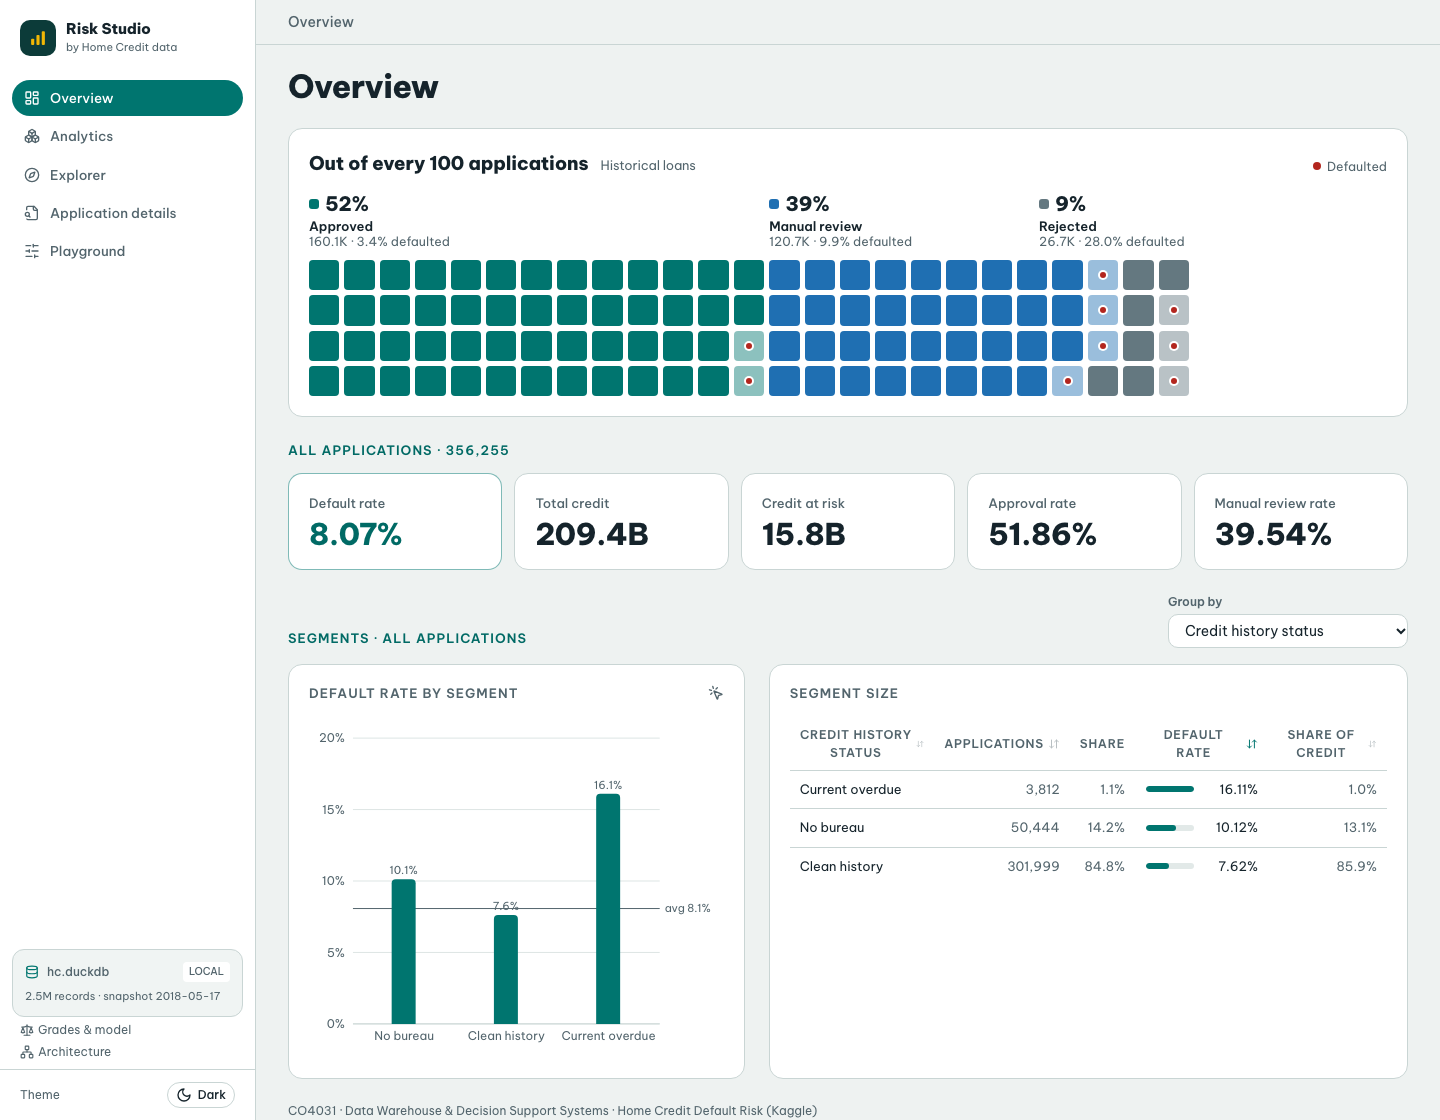
\includegraphics[width=\textwidth]{images/page_overview.png}
	\caption{Trang tổng quan (\textbf{Overview})}
	\label{fig:page_overview}
\end{figure}

\subsection{Trang Analytics}
Trang \textbf{Analytics} minh họa các phép OLAP trên một khối dữ liệu và có hai thẻ: \textbf{Cube} và \textbf{SQL queries}. Hình~\ref{fig:page_analytics} là thẻ \textbf{Cube} với khoảng thời gian theo tháng; trục thời gian dùng ngày nộp hồ sơ mô phỏng.

\medskip

Thẻ \textbf{Cube} gồm bốn phần:
\begin{itemize}[topsep=0pt, itemsep=1pt]
	\item \textbf{Thanh lọc:} Thanh \textbf{Cohort} nhận các điều kiện dạng thẻ nhỏ (\textit{chip}) qua nút \textbf{Add filter}, mỗi điều kiện gồm trường, toán tử và giá trị. Một điều kiện là phép cắt lát, nhiều điều kiện trên nhiều chiều là phép cắt khối.
	\item \textbf{Khoảng thời gian:} Nút \textbf{Interval} chọn Year, Quarter hoặc Month cho ba biểu đồ theo thời gian, tương ứng phép cuộn lên và khoan xuống. Trục thời gian dùng ngày nộp hồ sơ mô phỏng, nên dao động giữa các kỳ chỉ là nhiễu.
	\item \textbf{Bốn biểu đồ cố định:} \textbf{Applications over time} đếm hồ sơ theo quyết định. \textbf{Default rate over time} chỉ tính trên khoản vay lịch sử, nên dừng ở khoảng tháng 5/2017. \textbf{Grade mix over time} cho tỷ trọng hạng cuối, còn \textbf{Default rate by segment} so sánh các nhóm theo chiều chọn ở \textbf{Split by}.
	\item \textbf{Bảng Cube:} Người dùng chọn tối đa $2$ chiều hàng, $1$ chiều cột và một thước đo ở \textbf{Measure}. Các nút $\blacktriangle$/$\blacktriangledown$, $\times$, \textbf{Add dimension} và $\rightleftarrows$ thực hiện các phép ở Bảng~\ref{tab:olap-ui}. Bảng tô màu theo giá trị và có tổng phụ ở cột và dòng \textbf{All}.
\end{itemize}

Trong Hình~\ref{fig:page_analytics}, bảng \textbf{Cube} có hàng là năm nộp hồ sơ (mô phỏng), cột là hạng cuối và thước đo là \textbf{Default rate}. Tỷ lệ vỡ nợ tăng đều theo hạng: $0{,}6\%$ ở hạng A, $3{,}5\%$ ở hạng B, $8{,}3\%$ ở hạng C, $12{,}1\%$ ở hạng D và $28{,}0\%$ ở hạng E. Dòng 2018 để trống vì hồ sơ nộp năm đó là hồ sơ mới, chưa có kết quả.

\begin{figure}[H]
	\centering
	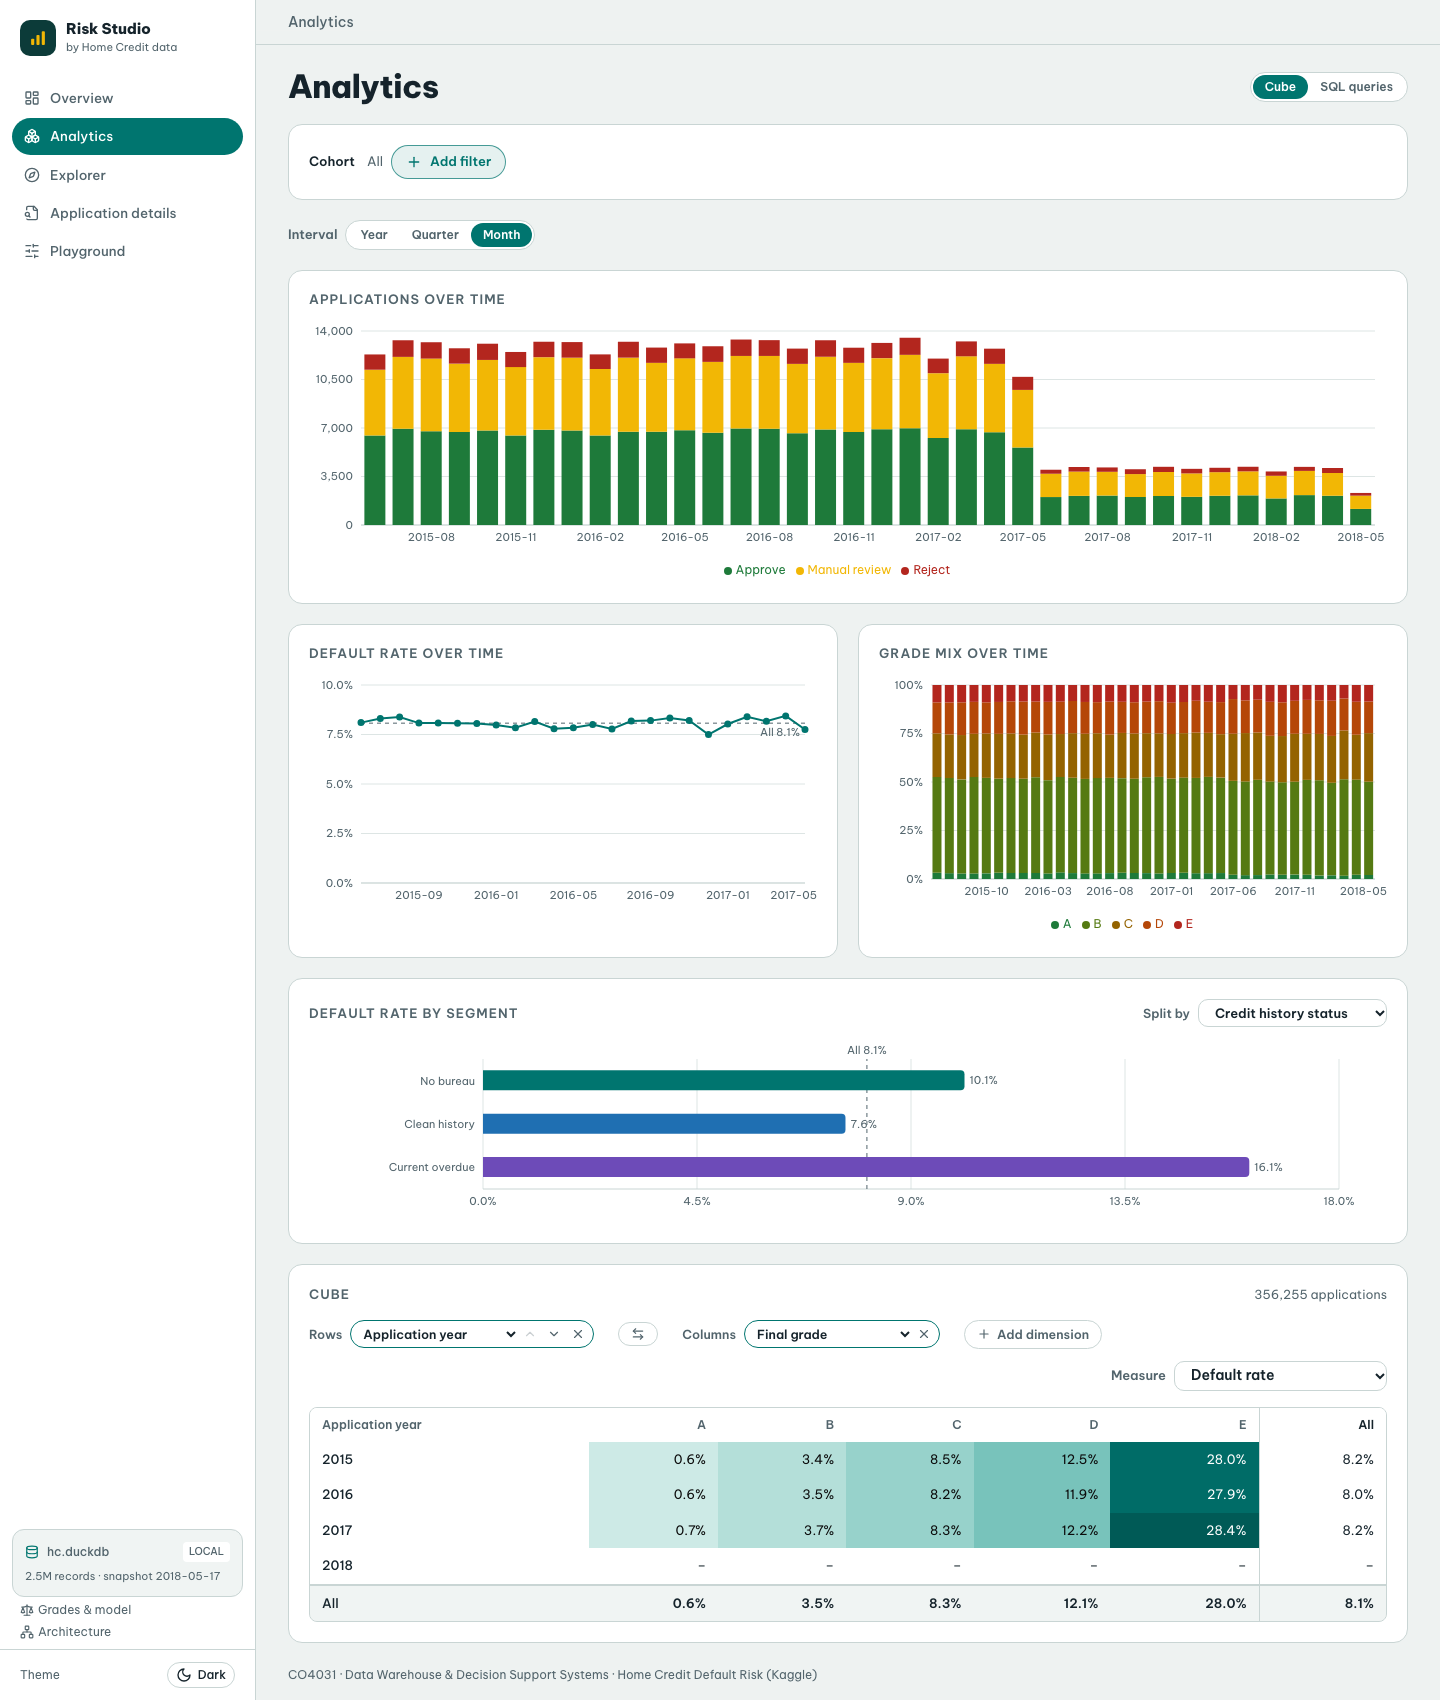
\includegraphics[width=\textwidth]{images/page_analytics.png}
	\caption{Trang phân tích (\textbf{Analytics}), thẻ \textbf{Cube}}
	\label{fig:page_analytics}
\end{figure}

Thẻ \textbf{SQL queries} chạy sáu truy vấn mẫu ở mục~\ref{sec:olap-scenarios}. Hình~\ref{fig:page_analytics_sql} cho thấy danh sách truy vấn bên trái và kết quả của truy vấn đang chọn bên phải. Nút \textbf{Show SQL} hiện câu lệnh SQL tương ứng.

\begin{figure}[H]
	\centering
	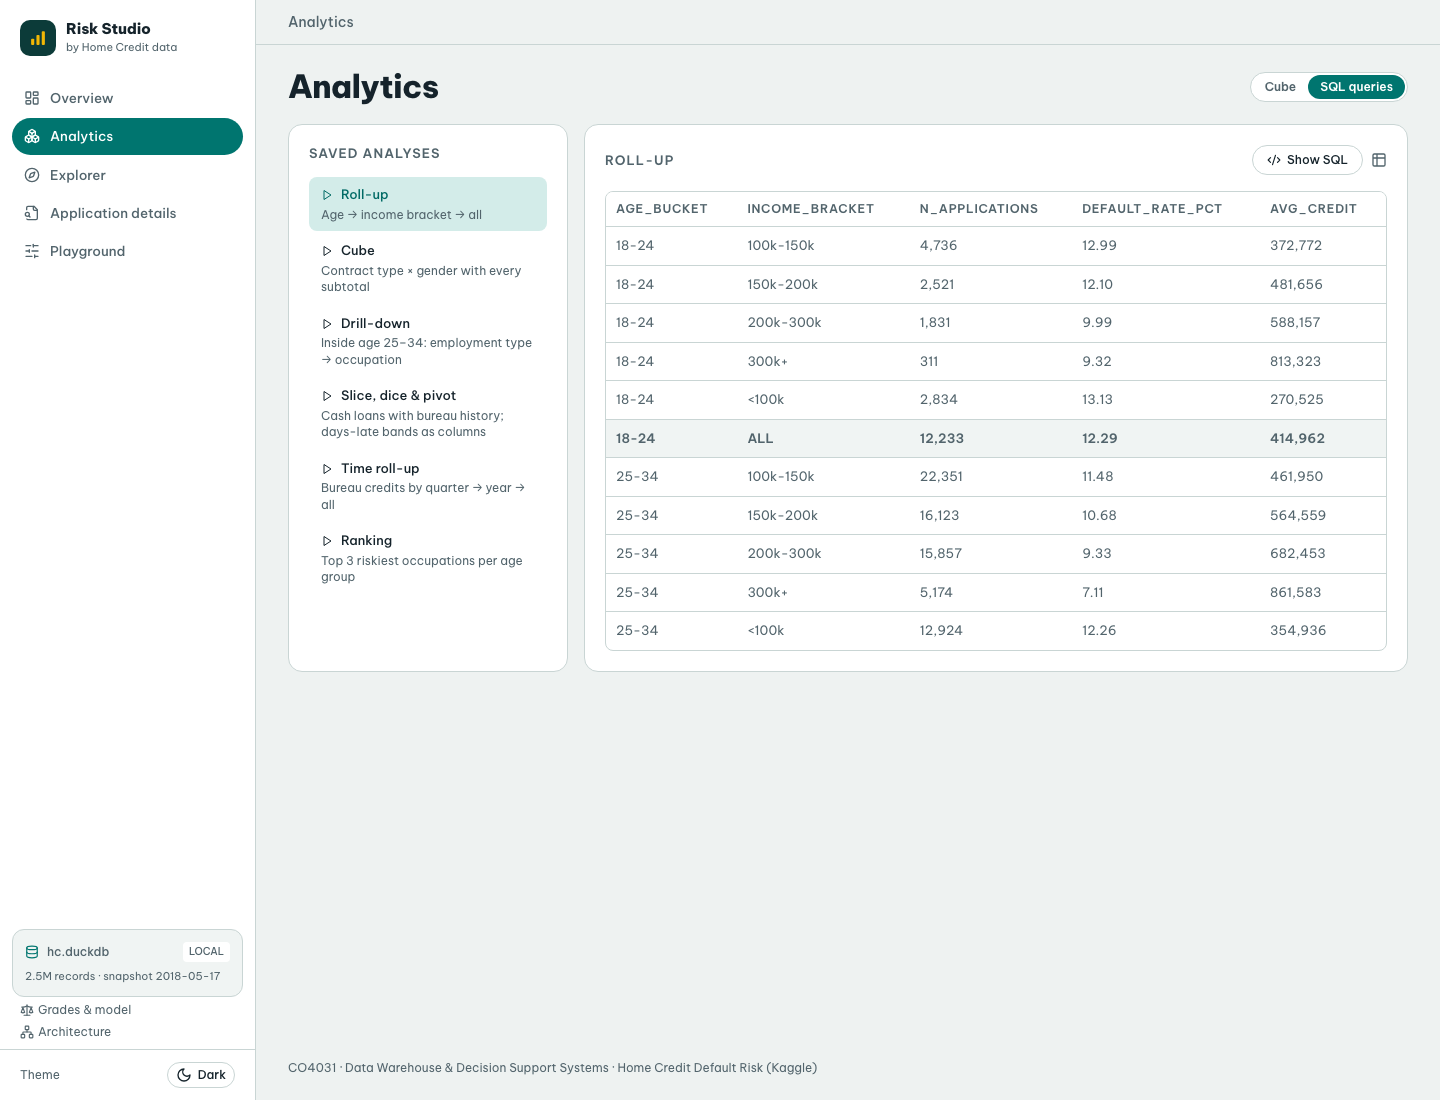
\includegraphics[width=\textwidth]{images/page_analytics_sql.png}
	\caption{Trang phân tích (\textbf{Analytics}), thẻ \textbf{SQL queries}}
	\label{fig:page_analytics_sql}
\end{figure}

\subsection{Trang Explorer}
Trang \textbf{Explorer} trả lời câu hỏi: rủi ro đang dồn vào phân khúc nào, và chính sách nào xử lý được phân khúc đó. Trang so một nhóm hồ sơ do người dùng chọn với mọi hồ sơ. Hình~\ref{fig:page_explorer} là trang khi chưa có điều kiện lọc.

\begin{figure}[H]
	\centering
	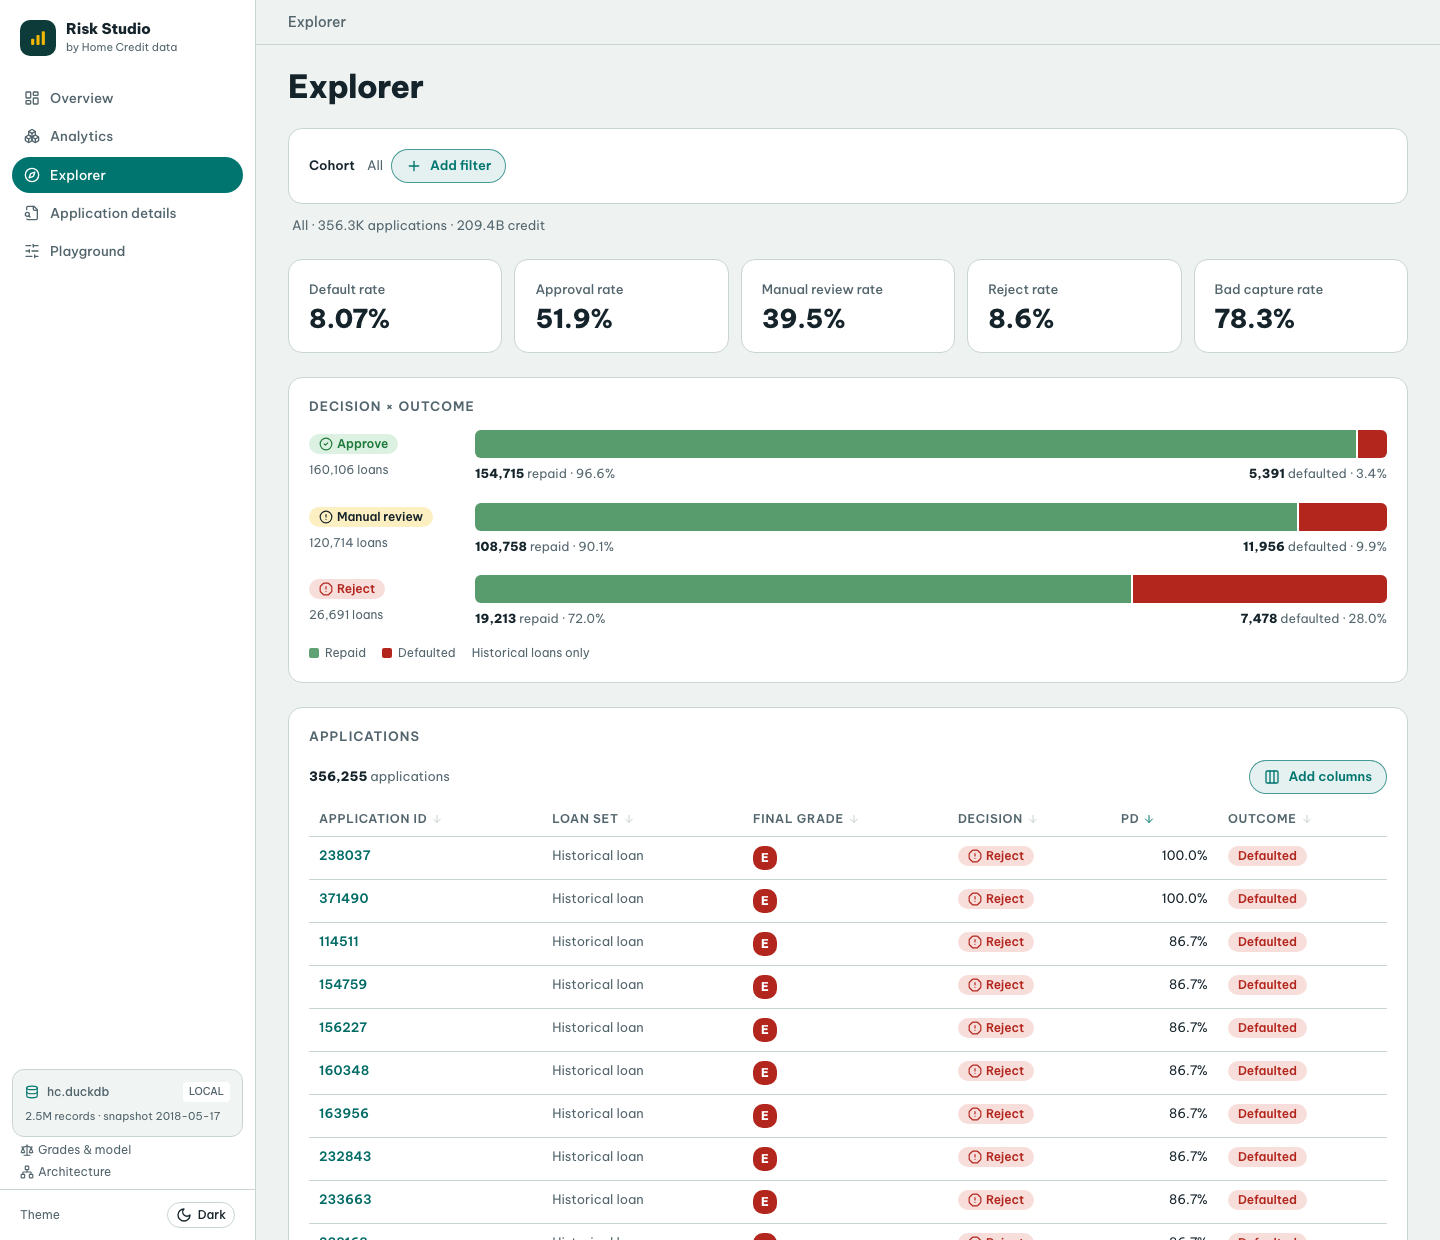
\includegraphics[width=\textwidth]{images/page_explorer.png}
	\caption{Trang khám phá (\textbf{Explorer})}
	\label{fig:page_explorer}
\end{figure}

Trang có bốn phần:
\begin{itemize}[topsep=0pt, itemsep=1pt]
	\item \textbf{Bộ lọc nhóm:} Thanh \textbf{Cohort} dùng cùng mô hình điều kiện với trang \textbf{Analytics}. Các điều kiện nối bằng phép hội (AND) và được lưu trên URL. Danh sách trường có cả ngày nộp, ngày có kết quả và số tháng tới kết quả, đều là dữ liệu mô phỏng.
	\item \textbf{Chỉ số của nhóm:} Năm ô gồm \textbf{Default rate}, \textbf{Approval rate}, \textbf{Manual review rate}, \textbf{Reject rate} và \textbf{Bad capture rate}. \textbf{Default rate} và \textbf{Bad capture rate} chỉ tính trên khoản vay lịch sử; ba tỷ lệ quyết định tính trên mọi hồ sơ. Khi có điều kiện lọc, mỗi ô ghi thêm chênh lệch so với mọi hồ sơ, tính bằng điểm phần trăm.
	\item \textbf{Quyết định và kết quả:} Khung \textbf{Decision $\times$ outcome} đếm số khoản vay lịch sử trả tốt và vỡ nợ trong từng nhóm quyết định.
	\item \textbf{Danh sách hồ sơ:} Bảng \textbf{Applications} phân trang, sắp xếp được và cho thêm cột qua nút \textbf{Add columns}. Bấm một dòng mở trang \textbf{Application details} của hồ sơ đó.
\end{itemize}
Khi chưa lọc, \textbf{Bad capture rate} là $78{,}3\%$: chính sách hiện hành chuyển thẩm định hoặc từ chối $19.434$ trên $24.825$ khoản vỡ nợ. Nhóm Duyệt có $160.106$ khoản vay lịch sử, trong đó $5.391$ khoản vỡ nợ ($3{,}4\%$). Nhóm Thẩm định thêm có $120.714$ khoản với $11.956$ khoản vỡ nợ ($9{,}9\%$). Nhóm Từ chối có $26.691$ khoản với $7.478$ khoản vỡ nợ ($28{,}0\%$).

Trang \textbf{Architecture} hiển thị các sơ đồ thiết kế của hệ thống ở giao diện sáng hoặc tối và cho tải về dạng SVG.
\endgroup
